\section{Homeomorphisms and distinguishability}
\label{homeomorphisms}
Often in mathematics, when talking about objects as certains things coming with certain structures, we want to be able to say when two objects are ``the same''. Consider for instance the two topological spaces $X = \{ 1 , 2 , 3 \}$ and $Y = \{ 4, 5, 6 \}$ with the topologies
\begin{align*}
  \calT_X &= \{ \emptyset, \{1 \}, \{ 2 \}, \{ 1, 2 \}, \{1,2,3\} \}, \\
  \calT_Y &= \{ \emptyset, \{4 \}, \{ 5 \}, \{ 4, 5 \}, \{4,5,6\} \}.
\end{align*}
These spaces are not particularly different for if we identify $1 \leftrightarrow 4$, $2 \leftrightarrow 5$, $3 \leftrightarrow 6$, we have no way to tell them apart. This notion of being the same is made precise in the definition of a ``homeomorphism'' below.

The well-educated mathematics student will have likely come across this general idea before: we consider two vector spaces the same if there is a linear isomorphism from one to the other, we consider algebraic objects such as groups and rings the same if they are isomorphic, and if all we know about two given sets is that they are in bijection, we may as well treat them as the same. This language of ``objects'' being ``the same'' is unified in the branch of mathematics called \word{category theory}{kategoriteori}, sometimes referred to as \emph{abstract nonsense}\index{abstract nonsense}. We will be discussing category theory in any detail in these notes, but it is useful to be aware of its existence.

\subsection{Homeomorphisms}
In the example above, we notice that crucial property of two topological spaces that ``are the same'' is that they are in bijection and have the same open sets. This leads to the following definition.
\begin{defn}
  A bijection $f : X \to Y$ between two topological spaces is called a \word{homeomorphism}{homeomorfi} if $f$ and its inverse $f^{-1}$ are continuous. In this case, we say that $X$ and $Y$ are \word{homeomorphic}{homeomorfa} and we write $X \simeq Y$.
\end{defn}
Equivalently, since a bijection $f$ always satisfies $f = (f^{-1})^{-1}$, one could define a homeomorphism to be a bijection such that $f(U)$ is open whenever $U$ is. Notice also that $\simeq$ satisfies the property of an equivalence relation.
\trans{homeomorphism}{homeomorfi}\trans{homeomorphic}{homeomorfa}
\begin{example}
  In the example in the beginning of this section, the bijection $f : X \to Y$ given by $f(1) = 4$, $f(2) = 5$, $f(3) = 6$ is a homeomorphism.
\end{example}
\begin{example}
  Let $f : (-1 , 1) \to \bbR$ be the bijective map
  \[
    f(x) = \tan \left( \frac{\pi x}{2} \right)
  \]
  whose inverse is $f^{-1}(x) = \tfrac{2}{\pi} \arctan x$. Then both $f$ and $f^{-1}$ are continuous so $(-1,1)$ and $\bbR$ are isomorphic.
\end{example}
From the above example we conclude that two spaces that we are otherwise familiar with and think of as different may turn out to be the same from the viewpoint of topology. Roughly, since we don't care about the scale of $(-1,1)$ but only its open sets, we are able to stretch it as much as we please, and end up with something like $\bbR$
\begin{badjoke}
  Let $A$ be a typical topologist. Then $A$ is not able to tell the difference between her coffee mug and her donut.
\end{badjoke}
\begin{proof}
  The surfaces of the coffee mug and the donut are homeomorphic. See \url{https://upload.wikimedia.org/wikipedia/commons/2/26/Mug_and_Torus_morph.gif}.
\end{proof}
\begin{example}
  Let $B^n := B(0,1)$ be the unit ball in $\bbR^n$. Then $B^n \simeq \bbR^n$. This can be seen because the map $f : B^n \to \bbR^n$ given by
  \[
    f(x) = \frac{x}{1-\Abs{x}}
  \]
  is a continuous bijection with inverse
  \[
    f^{-1}(x) = \frac{x}{1+\Abs{x}}.
  \]
\end{example}
We will often be interested in functions that would be homeomorphisms if we were allowed to shrink the codomain appropriately.
\begin{defn}
  Let $X$ and $Y$ be topological spaces. A function $f: X \to Y$ is called an \word{embedding}{?} if $f : X \to f(X)$ is a homeomorphism; here $f(X)$ has the subspace topology from $Y$.
\end{defn}
\begin{example}
  If $X$ is a topological space and $Y \subset X$ a subspace, then the inclusion $\iota : Y \to X$ given by $\iota(x) = x$ is an embedding.
\end{example}

\subsection{Topological invariants}
Above, we have talked about what it means for two topological spaces to be the same. Often, one will be interested in the converse question of telling two topological spaces apart. As such, we consider topological spaces different if they are non-homeomorphic; for instance, if $X = \{a,b\}$ then we obtain two different topological spaces by equipping it with the trivial and the discrete topology.

\begin{defn}
  Let \textbf{Top} denote the collection of \emph{all} topological spaces. A \emph{topological invariant}, sometimes called a \emph{topological property}, is a function $f$ defined on \textbf{Top} so that if $X \simeq Y$, then $f(X) = f(Y)$.
\end{defn}
The important thing to note is that if $f$ is a topological invariant and $f(X) \not= f(Y)$, then $X$ and $Y$ are not homeomorphic. Thus we are lucky enough, we can use topological invariants to tell topological spaces apart.
\begin{example}
  Let $f : \textbf{Top} \to \{ \text{yes}, \text{no} \}$ be the function given by answering the question ``is $X$ Hausdorff?'' That is
  \[
    f(X) = \begin{cases} \text{yes}, &\text{ if $X$ is Hausdorff,}\\ \text{no}, &\text{ if $X$ is not Hausdorff.} \end{cases}
  \]
  Then $f$ is a topological invariant: if $X \simeq Y$ and $X$ is Hausdorff, then so is $Y$. For this reason, the property of being Hausdorff is often called a topological property. Again, one can turn this around and say that if $X$ is Hausdorff but $Y$ is not, then $X$ and $Y$ are not homeomorphic. Similarly, being $T_0$ or $T_1$ are topological properties. As is being first-countable and any other property that is defined using only in terms of open sets.
\end{example}

We will encounter many other topological properties later on, one of the most important ones being the fundamental group, which is to be introduced in Section~\ref{homotopy}.

\subsection{The $n$-dimensional sphere}
\begin{defn}
  The \emph{$n$-sphere} is the set
  \[
    S^n = \{ x \in \bbR^{n+1} \mid \Abs{x} = 1 \} \subset \bbR^{n+1}
  \]
  with the subspace topology from $\bbR^{n+1}$.
\end{defn}
\begin{prop}
  Let $p = (0,0,\dots,0,1) \in S^n$ be the ``north pole''. Then $S^n \setminus \{p\} \simeq \bbR^n$.
\end{prop}
\begin{proof}
  We will construct a homeomorphism explicitly, leaving some of the details to the reader. Let $x = (x_1, \dots, x_{n+1}) \in S^n \setminus \{ p \}$ so that $x_{n+1} \not= 1$. We then define the \word{stereographic projection}{stereografisk projektion} of $x$ by
  \[
    \Pi(x) = \Pi(x_1,\dots,x_n,x_{n+1}) = \frac{1}{1-x_{n+1}} (x_1, \dots, x_n) \in \bbR^n.
  \]
  Geometrically, if one draws a straight line through $x$ and $p$, then its intersection with $\bbR^n \times \{0 \}$ will be the point $(\Pi(x),0)$. Now $\Pi$ is continuous because each of its components are (use Proposition~\ref{props-subspace-top} and Lemma~\ref{universal-inclusion-lemma}), and one can check that it has an inverse $g : \bbR^n \to S^n \setminus \{p \}$ given by
  \[
    g(y_1, \dots, y_n) = (t(y) y_1, \dots, t(y)y_n, 1-t(y)),
  \]
  where $t(y) = 2/(1+\Abs{y}^2)$.
\end{proof}
\begin{rem}
  If $q = (0,\dots,0,-1) \in S^n$ is the south pole, then the map $(x_1, \dots, x_n,x_{n+1}) \mapsto (x_1,\dots,x_n,-x_{n+1})$ is a homeomorphism from $S^n \setminus \{p\}$ to $S^n \setminus \{ q \}$, so we also have that $S^n \setminus \{ q \}$ is homeomorphic with $\bbR^n$. More generally, one can show $S^n \setminus \{x\} \simeq \bbR^n$ for all $x \in S^n$.
\end{rem}
\begin{example}
  Let $f : [0,1) \to S^1$ be the map $f(x) = (\cos (2\pi x), \sin(2\pi x))$. Then $f$ is a bijection with inverse $f^{-1}(x,y) = \arcsin(y)/(2\pi)$. Moreover, $f$ is continuous by Proposition~\ref{props-subspace-top} and Lemma~\ref{universal-inclusion-lemma}. Now $U = [0,\tfrac{1}{2})$ is open in $[0,1)$ (recall Example~\ref{weird-opens-subspace-example}) but $f(U)$ is not open in $S^1$ (this is intuitively clear but of course requires a formal proof -- try to cook one up!). Thus $f$ is not a homeomorphism, even though it is a continuous bijection.
\end{example}

\subsection{The quotient topology}
The quotient topology provides us with yet another way of making new topological spaces out of existing ones.

\begin{defn}
  Let $X$ and $Y$ be topological spaces, and let $p : X \to Y$ be a surjective map. Then $p$ is called a \word{quotient map}{?} if it has the property that $U \subset Y$ is open if and only if $p^{-1}(U) \subset X$ is open.
\end{defn}
\trans{quotient map}{?}
Notice that a quotient map is automatically continuous, but it need not be a homeomorphism since it is not necessarily injective; indeed we will be mostly interested in the cases where it's not.

One motivation for studying quotient maps is that they allow us to glue topological spaces together to obtain new ones. In practice, one does this by introducing an equivalence relation whose equivalence classes correspond to the points that we want to glue. An equivalent description is given in terms of general quotient a bit later in this section.

\begin{defn}
  \label{def-quotient-topology}
  Let $X$ be a topological space with an equivalence relation $\sim$. Let $p : X \to X/\!\sim$ be the map $p(x) = [x]$. The \word{quotient topology}{?} on $X/\!\sim$ is the topology defined by saying that $U \subset X/\!\sim$ is open if $p^{-1}(U) \subset X$ is open. In other words, it is the unique topology that forces $p$ to be a quotient map.
\end{defn}
\trans{quotient topology}{?}

\begin{example}
  \label{collapse-space}
  We can use the quotient topology to collapse parts of a topological space to a point. Let $U \subset X$ be any subset in a topological space and define an equivalence relation $\sim_U$ on $X$ by $x \sim y$ if $x = y$ or $x,y \in U$. The equivalence class of a point $x$ is
  \[
    [x]_U = \begin{cases} \{x\},& \text{if $x \notin U$,} \\ U,& \text{if $x \in U$.} \end{cases}
  \]
  Intuitively speaking, in $X/\!\sim_U$ we have collapsed the set $U$ to consist of a single point while we have left the rest of the space unchanged.
\end{example}
We will use the notation $X/U = X/\!\sim_U$ for the space obtained using the equivalence relation of Example~\ref{collapse-space}.
\begin{example}
  Let us see what the above space means for the topology of the space. Let $X = [-1,1]$ and let $U = \{-1,1\}$ be the endpoints of the interval. One can then show that $X/U \simeq S^1$: that is, we can tie together the ends of the interval to obtain a circle. We will show this precisely in Example~\ref{circle-from-interval}.
  
  More generally, if $X = B^n \subset \bbR^n$ is the closed unit ball, then the $(n-1)$-sphere $S^{n-1} \subset B^n$ forms the boundary of $B^n$ in $\bbR^n$. Now if $U = S^{n-1}$ one can show that $B^n/S^{n-1} \simeq S^n$. Picturing the case $n = 2$ is probably helpful.
\end{example}
The following result allows us to determine continuity of functions defined on quotient spaces in terms of the spaces they originate from.
\begin{lem}
  \label{universal-property-quotients}
  Let $X$ and $Y$ be a topological spaces, and let $\sim$ be an equivalence relation on $X$. Suppose that $f : X \to Y$ is a map with the property that $x \sim y$ implies that $f(x) = f(y)$. There then exists a unique map $g : X /\!\sim \to Y$ so that $f = g \circ p$, where $p : X \to X/\!\sim$ is the canonical surjection $p(x) = [x]$. Moreover, $g$ is continuous if and only if $f$ is.
\end{lem}
\begin{proof}
  Let us first define a $g$ that works: let $[x] \in X/\!\sim$ for $x \in X$. We then define $g([x]) = f(x) \in Y$. The condition on $f$ ensures that $g$ is well-defined, i.e. that if $[x] = [y]$, then $g([x]) = g([y])$. Now by construction $f = g \circ p$. We will show that $g$ is continuous if and only if $f$ is, and that $g$ is the only map that satisfies $f = g \circ p$.
  
  Let us start with the latter; assume that there is a map $g' : X/\!\sim \to Y$ with $f = g' \circ p$. We then have
  \[
    g([x]) = f(x) = (g' \circ p)(x) = g'(p(x)) = g'([x])
  \]
  for all $x \in X$ so in particular $g([x]) = g'([x])$ for all $[x] \in X/\!\sim$.
  
  Now if $g$ is continuous, so is $f$ since it is a composition of continuous maps.
  
  Assume that $f$ is continuous and let $V \subset Y$ be open. Then $f^{-1}(V) = p^{-1}(g^{-1}(V))$ is open, but the quotient topology is defined to ensure that $p$ is a quotient map, which implies that $g^{-1}(V)$ is open, so $g$ is continuous.
\end{proof}
Above we have seen how equivalence relations can be used to define interesting quotient spaces. We will now turn to a result which says that all such quotient spaces may be described in terms of quotient maps.

More precisely, let $f :X \to Y$ be a surjective map. Then we define an equivalence relation $\sim_f$ by requiring that $x \sim_f y$ if and only if $f(x) = f(y)$. With this relation, the equivalence classes are exactly the sets in $X$ of the form $f^{-1}(\{p\})$ for $p \in Y$, and there is a bijection $g: X/\!\sim_f \to Y$ given by $g(f^{-1}(\{p\})) = p$. Notice that we need $f$ to be surjective for this construction to work.
\begin{prop}
  \label{quotients-are-equivalence-classes}
  Let $X$ and $Y$ be topological spaces, let $f : X \to Y$ be a surjective map, and let $g : X/ \!\sim_f \to Y$ be the bijection defined by $f^{-1}(\{p\}) \mapsto p$. If $f$ is a quotient map, then $g$ is a homeomorphism.
\end{prop}
\begin{proof}
  It follows from Lemma~\ref{universal-property-quotients} that $g$ is continuous, since $f$ is. Let $U \subset X/\!\sim_f$ be an open set, and let us show that $g(U)$ is open in $Y$ by showing that $g(U) = f(p^{-1}(U))$ which is open since $f$ is a quotient map. If $y \in g(U)$ there is an $[x] \in U$ so that $y = g([x]) = g(p(x)) = f(x)$, so $y \in f(U)$. Likewise, if $y \in f(p^{-1}(U))$, there is an $x \in p^{-1}(U)$ so that $f(x) = y$. This says that $[x] \in U$ and $g([x]) = f(x) = y$, so $y \in g(U)$.
\end{proof}
\begin{rem}
  In general, if $f : X \to Y$ is a surjection, and $(X,\calT_X)$ is a topological space, it is customary to define the quotient topology $\calT_Y$ on $Y$ by
  \[
    \calT_Y = \{ U \subset Y \mid f^{-1}(U) \in \calT_X \}.
  \]
  Then $Y$, with its quotient topology $\calT_Y$ is homeomorphic to $X/\!\sim_f$ with its quotient topology (from Definition~\ref{def-quotient-topology}).
\end{rem}
\begin{example}
  \label{circle-from-interval}
  Let us show that $[0,1]/\{0,1\}$, with the quotient topology, is homeomorphic to $S^1$. Let $f : [0,1] \to S^1$ be the map $f(x) = (\cos(2\pi x), \sin(2\pi x))$. Then $f(x) = f(y)$ if and only if $x = y$ or either $x=1,y=0$ or $x=0,y=1$. This implies that $[0,1]/\!\sim_f\, = [0,1]/\{0,1\}$. As before, $f$ is continuous, and $f$ is clearly surjective, so the induced map $g : [0,1]/\!\sim_f \,\to S^1$ is a homeomorphism by Proposition~\ref{quotients-are-equivalence-classes}.
\end{example}
\begin{example}
  Another way of viewing the same example is as follows: let $\sim$ be the equivalence relation on $\bbR$ given by $x \sim y$ if $x-y \in \bbZ$. Define $f : \bbR \to S^1$ by $f(x) = (\cos(2\pi x), \sin(2\pi x))$ just like above. Then $f(x) = f(y)$ if and only if $x \sim y$, so $\sim \,=\, \sim_f$. This implies that $\bbR/\sim$ is homeomorphic to $S^1$.
  
  Be aware that the space $\bbR/\!\sim$ is often denoted $\bbR/\bbZ$, but that this notation does \emph{not} agree with the one from Example~\ref{collapse-space}. This somewhat unfortunate coincidence comes from the fact that both $\bbR$ and $\bbZ$ are \emph{groups} of which one can form a group quotient. One can combine the study of groups and topological spaces into the study of topological groups. We will not be dealing with those, but the interested reader should check out the end of \cite[\S 22]{Mun}
\end{example}
\begin{example}
  \label{torus-example-gluing}
  Another important example is the so-called $2$-torus $T^2$, which should be familiar to those that are old enough to know the 1979 arcade shooter Asteroids. It is obtained by gluing together opposing sides of a rectangle $X=[0,1] \times [0,1]$. That is, define an equivalence relation $\sim$ on $X$ by $x \sim y$ of $x = y$, or $x=(p,0),y=(p,1)$, or $x=(0,p),y=(1,p)$, see Figure~\ref{fundamental-polygon-torus}. Just like $[0,1]/\{0,1\} \simeq S^1$, one can show that $X /\!\sim$ is homeomorphic to a circle of circles, $S^1 \times S^1$; we refer to \cite[\S 22]{Mun} where this is done by examining the open sets in both spaces. See Figure~\ref{figure-torus} for an illustration of the resulting space.
  
  More generally, we will also be considering the $n$-torus $T^n$, which we will simply define to be the product $T^n = S^1 \times \cdots \times S^1$ of $n$ copies of $S^1$.
\end{example}
\begin{figure}
\centering
\begin{minipage}{.5\textwidth}
  \centering
  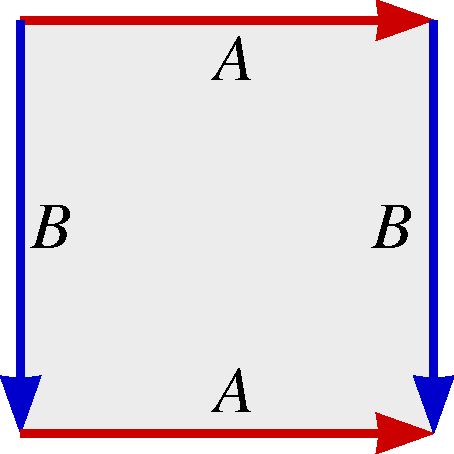
\includegraphics[width=.4\linewidth]{images/fundamental-polygon-torus}
  \caption{Illustration of $X = [0,1] \times [0,1]/\sim$.}
  \label{fundamental-polygon-torus}
\end{minipage}%
\begin{minipage}{.5\textwidth}
  \centering
  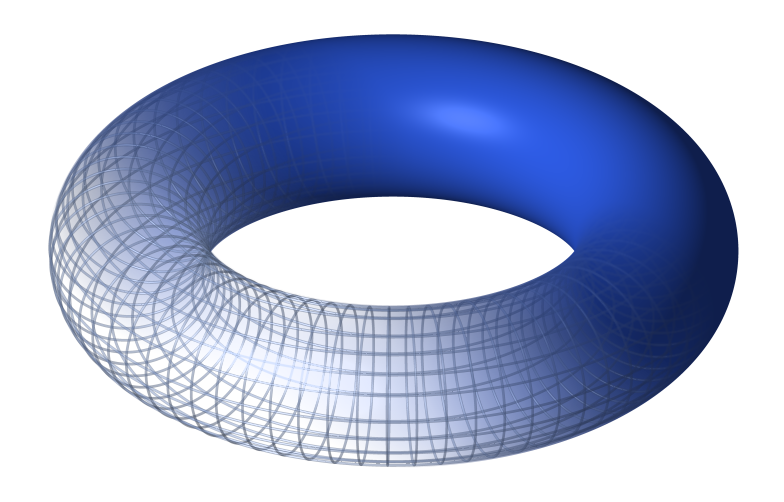
\includegraphics[width=.5\linewidth]{images/figure-torus}
  \caption{The resulting space $S^1 \times S^1$.}
  \label{figure-torus}
\end{minipage}
\end{figure}
\trans{real projective space}{?}\trans{Klein bottle}{Kleinflaska}
\begin{example}
  Consider again the $X = [0,1] \times [0,1]$. One could have chosen to identify the opposite sides in various other ways to obtain important spaces. In Figure~\ref{fundamental-polygon-projective} and Figure~\ref{fundamental-polygon-klein} two such spaces are shown. The former is the so-called \word{real projective plane}{?} and the latter is the \word{Klein bottle}{Kleinflaska}. The glued-together Klein bottle can be pictured as in Figure~\ref{figure-klein}.
\end{example}
\begin{figure}
\centering
\begin{minipage}{.45\textwidth}
\begin{minipage}{.95\textwidth}
  \centering
  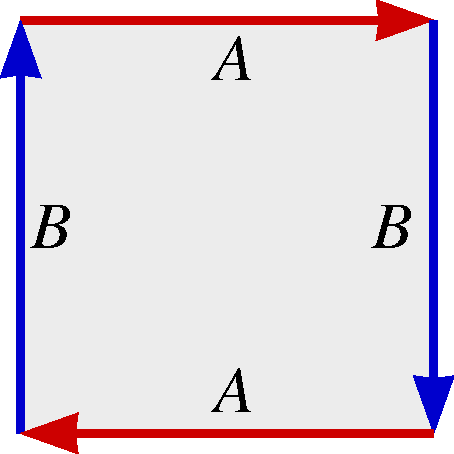
\includegraphics[width=0.5\linewidth]{images/fundamental-polygon-projective}
  \caption{Gluing the real projective plane.}
  \label{fundamental-polygon-projective}
\end{minipage}\\
\begin{minipage}{.95\textwidth}
  \centering
  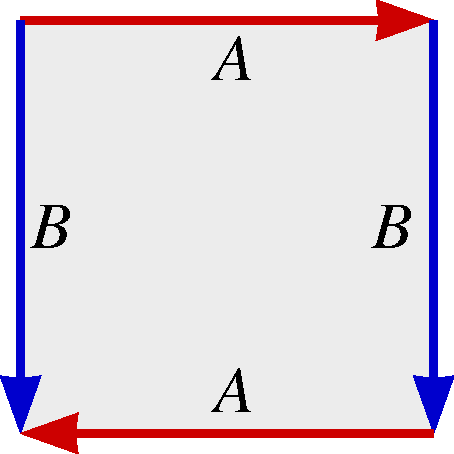
\includegraphics[width=0.5\linewidth]{images/fundamental-polygon-klein}
  \caption{Gluing the Klein bottle.}
  \label{fundamental-polygon-klein}
\end{minipage}

\end{minipage}
\begin{minipage}{.45\textwidth}
  \centering
  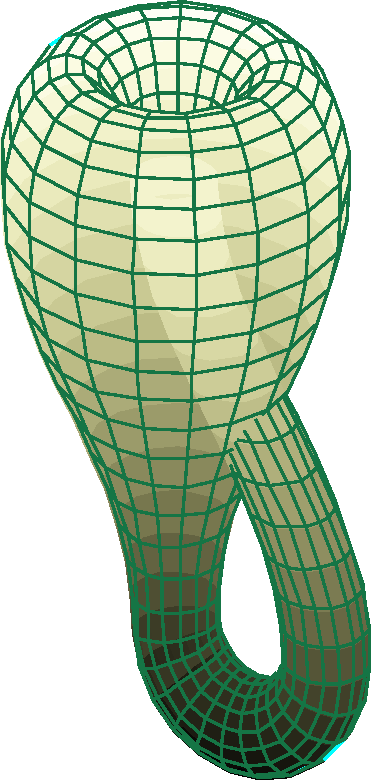
\includegraphics[width=.4\linewidth]{images/figure-klein}
  \caption{The Klein bottle.}
  \label{figure-klein}
\end{minipage}
\end{figure}
\begin{example}
  Finally, an important example is the following generalisation of Example~\ref{torus-example-gluing}: notice that we can describe the gluing pattern for the torus by starting at a corner of the square and taking note of the edges that we meet, together with their orientation. For instance, if we begin in the upper left corner of Figure~\ref{fundamental-polygon-torus} and move clockwise, we encounter the edges $ABA^{-1}B^{-1}$, where we use inverses to denote the orientations of the edges. Similarly, the gluings for the projective plane and the Klein bottle could be described as $ABAB$ and $ABAB^{-1}$ respectively.
  
  Now, consider a $4n$-gon $X_n$, $n > 0$, and glue together pairs of edges of the boundary according to the rule
  \[
    A_1 B_1 A_1^{-1} B_1^{-1} A_2 B_2 A_2^{-1} B_2^{-1} \cdots A_n B_n A_n^{-1} B_n^{-1},
  \]
  so that for instance, for $n = 1$ we recover the torus example. The resulting space $X_n / \!\sim$ is called a ``surface with $n$ handles'', or a ``genus $n$ surface''. See Figures~\ref{genus-1-surface}--\ref{genus-3-surface} for the examples $n = 1, 2, 3$. How to obtain these pictures is described nicely in \cite[Sect.~3.3]{Fje}.
\end{example}
\begin{figure}
\centering
\begin{minipage}{.33\textwidth}
  \centering
  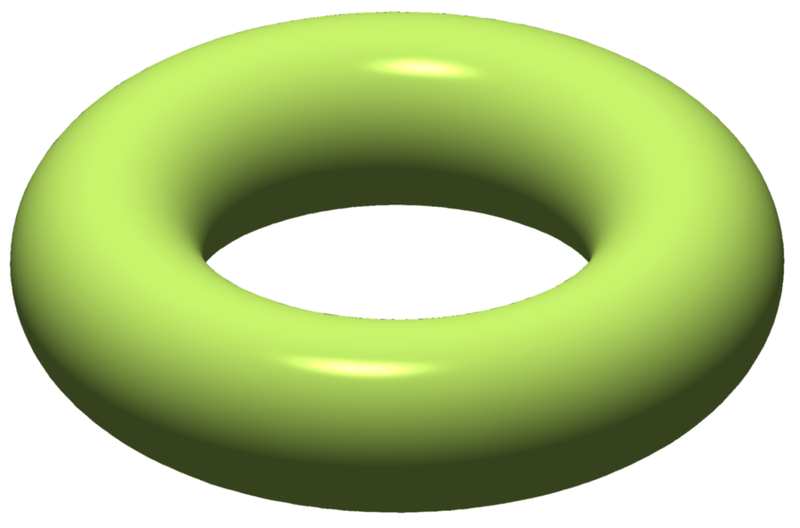
\includegraphics[width=.8\linewidth]{images/genus-1-surface}
  \caption{A genus $1$ surface.}
  \label{genus-1-surface}
\end{minipage}%
\begin{minipage}{.33\textwidth}
  \centering
  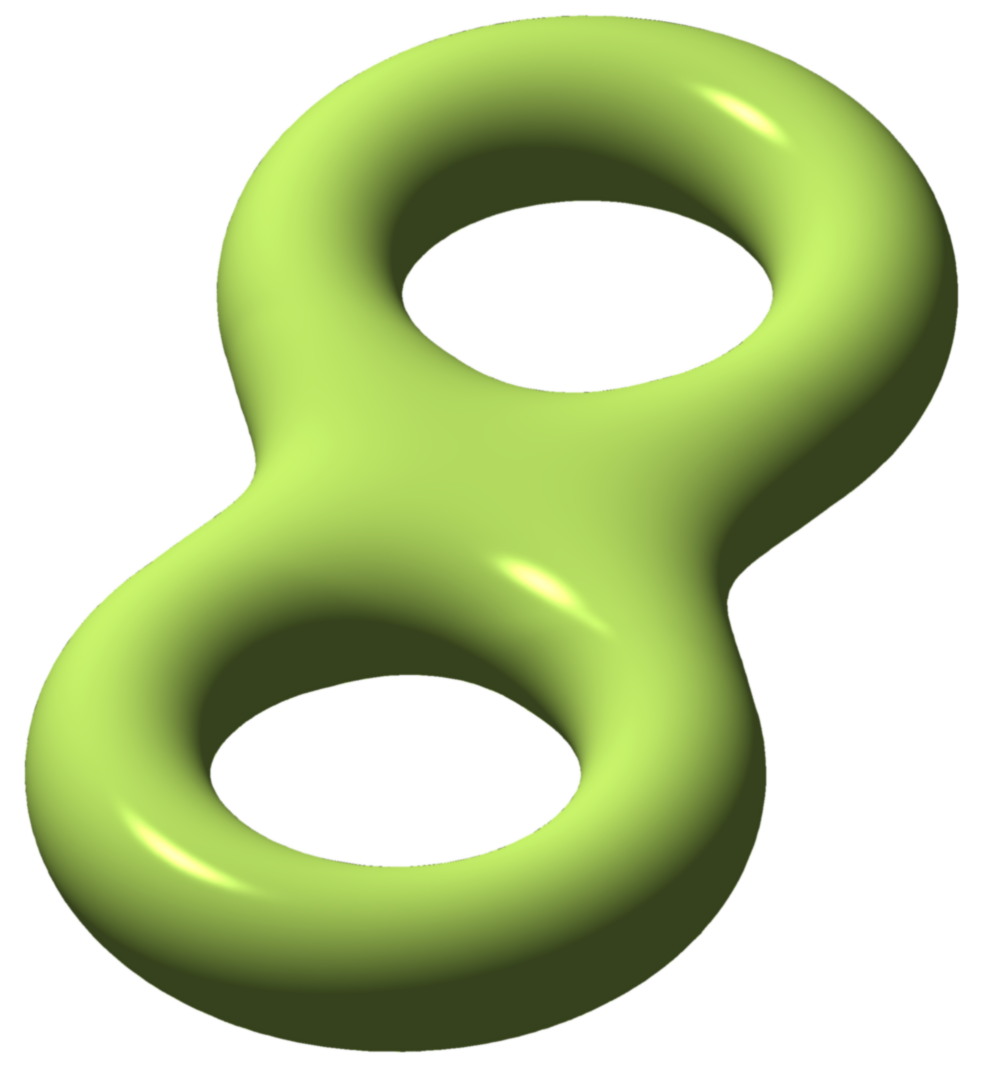
\includegraphics[width=.8\linewidth]{images/genus-2-surface}
  \caption{A genus $2$ surface.}
  \label{genus-2-surface}
\end{minipage}%
\begin{minipage}{.33\textwidth}
  \centering
  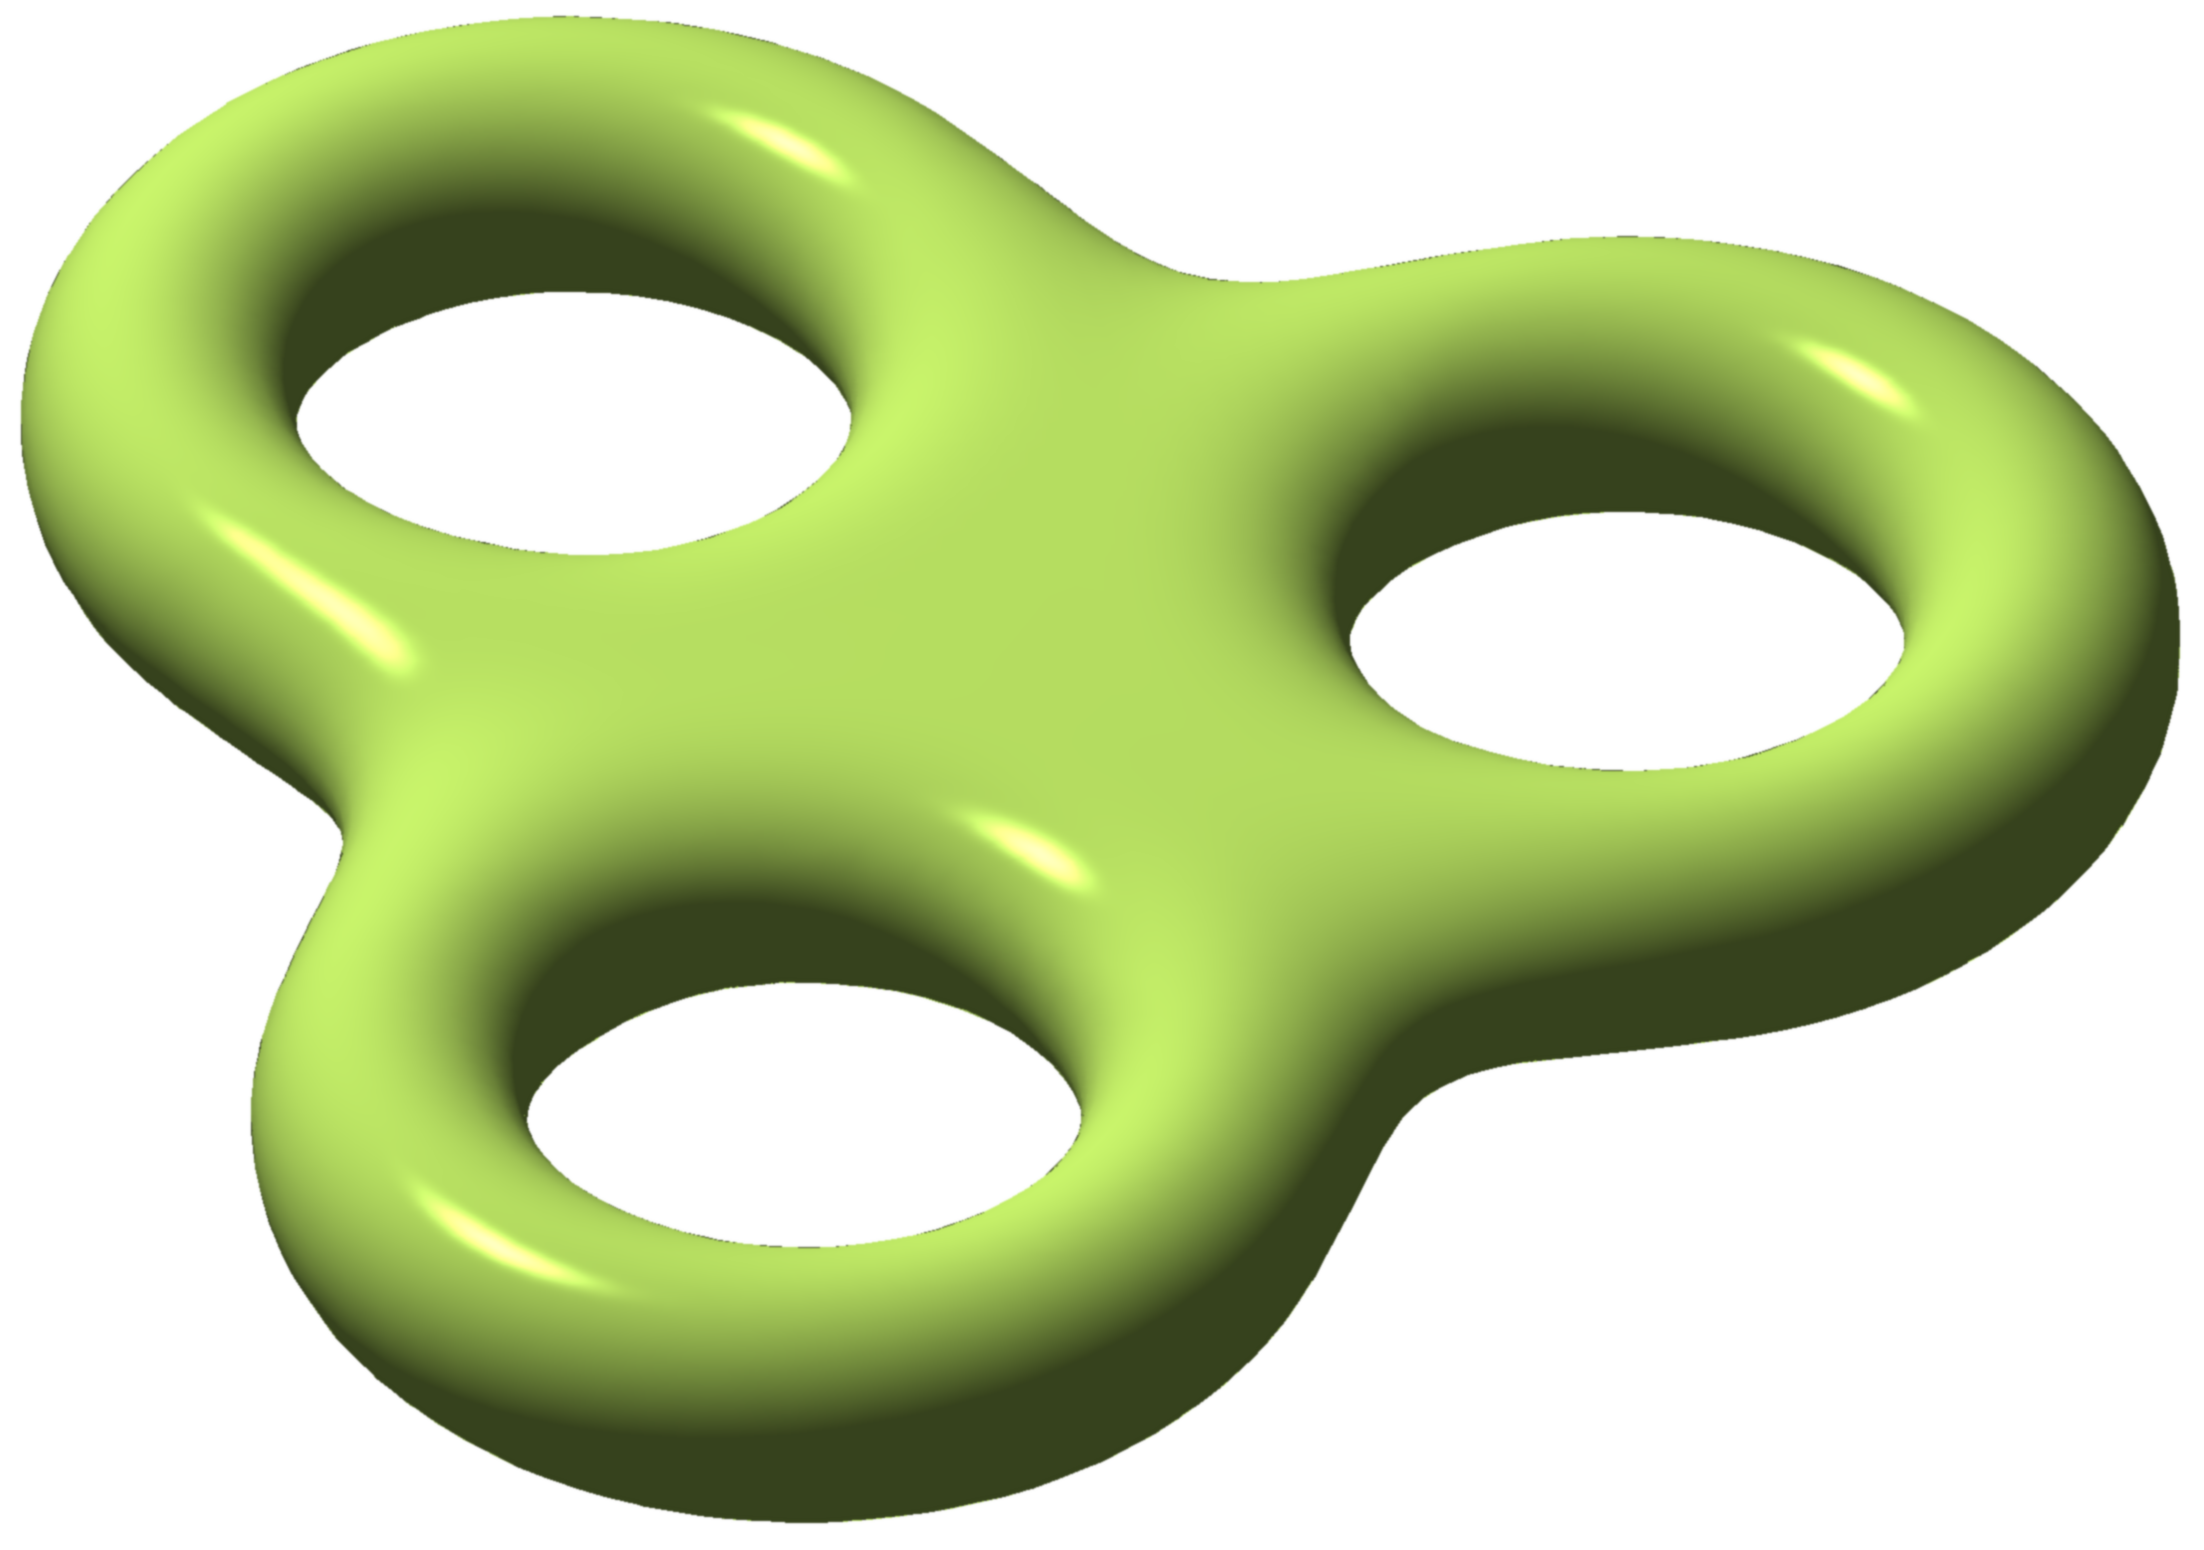
\includegraphics[width=.8\linewidth]{images/genus-3-surface}
  \caption{A genus $3$ surface.}
  \label{genus-3-surface}
\end{minipage}%
\end{figure}
